\subsection{Chapter 18 - Electric current}

\subsubsection{Overview}\label{chapter:current}

In this chapter, we introduce tools to model electric current, namely, the motion of charges inside a conductor. We will show how we can connect the microscopic motion of electrons to macroscopic quantities, such as current and voltage, that can be measured in the laboratory. We will also introduce the notion of resistance, as well as the resistor, a common component in electric circuits.

\begin{framed}
\textbf{Learning Objectives}\\
\begin{itemize}
\item Understand the differences in modelling conductors when charges are stationary or moving.
\item Understand how to define current and current density.
\item Understand the differences between resistance, resistivity, and conductivity.
\item Understand Ohm's Law.
\item Understand how to model how power is dissipated in a resistor.
\item Understand how to model alternating current.
\item Understand some elements of electrical safety.
\end{itemize}
\end{framed}

\begin{framed}
\textbf{Think About It}\\
Why is it safe to touch the $300000 {\rm V}$ terminal of a Van de Graaf generator, and not the $12 {\rm V}$ terminal of a car battery?\}

\begin{enumerate}
\item The Van de Graaf generator cannot sustain a large current.
\item The Van de Graaf generator produces alternating current.
\item The car battery produces $12 {\rm V}$ of alternating voltage.
\end{enumerate}

\begin{framed}
\textbf{Answer}\\
\begin{enumerate}
\item
\end{enumerate}
\end{framed}
\end{framed}

\subsubsection{Current}

In the preceding chapters, we examined ``electrostatic'' systems; those for which charges are not in motion. In electrostatic systems, the electric field inside of a conductor is zero (by definition, or charges would be moving, since they are free to move in a conductor). We argued that if charges are deposited onto a conductor, they would quickly arrange themselves into a static configuration (on the surface of the conductor).

To build a system that is not electrostatic, we could apply a fixed potential difference across the conductor. This would create an  electric field inside the conductor, causing the electrons to move. In general, this requires the formation of a circuit, whereby charges enter one end of the conductor and exit the other. The most simple circuit is constructed by connecting the two terminals of a battery to the ends of a conductor, as illustrated in Figure~\ref{fig:current:simplecircuit}.

\begin{figure}[!htbp]
\centering
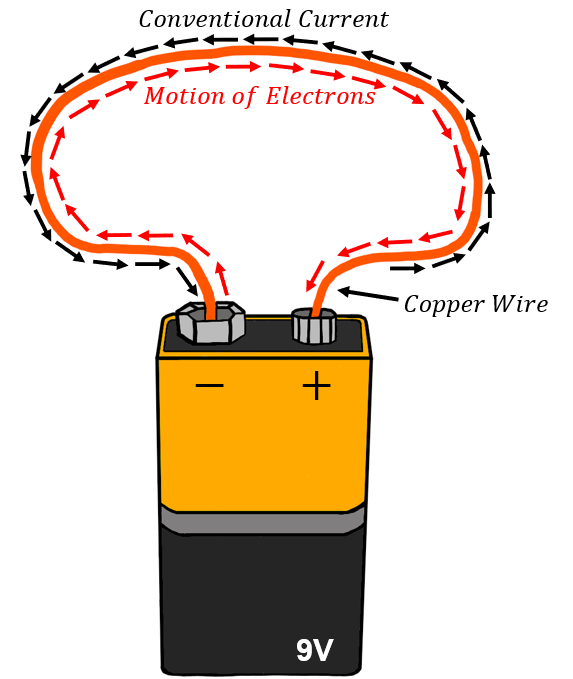
\includegraphics[width=0.4\linewidth]{files/simplecircuit-c553cfef088a33e4ea40ba088bf27fb7.png}
\caption[]{A simple circuit is created by connecting the terminals of a battery to a conducting material such as a copper wire. Note that while electrons flow from the negative to the positive terminal of the battery, conventional current is defined as if it were positive charges moving in the opposite direction.}
\label{fig:current:simplecircuit}
\end{figure}

A battery (as we will see in more detail in Section~\ref{chapter:circuits} is a device that provides a source of charges and a fixed potential difference. For example, a $9 {\rm V}$ battery has two terminals with a constant voltage of $9 {\rm V}$ between them.

``Electric current'' is defined to be the rate at which charges cross a given plane (usually a plane perpendicular to some conductor through which we want to define the current). We define current, $I$, as the total amount of charge, $\Delta Q$, that flows through any cross-section of the conductor during an amount of time, $\Delta t$:
\begin{equation}
\boxed{I=\frac{\Delta Q}{\Delta t}=\frac{dQ}{dt}}
\end{equation}
where we must take a derivative if the rate of flow is not constant in time. The S.I. unit of current is the Amp`ere ({\textbackslash}si\{A\}). In almost all cases, it is negative electrons that flow through a material. However, the current is defined to be in the direction of the flow of positive charges, as illustrated in Figure~\ref{fig:current:simplecircuit}. To distinguish that the current is in the direction opposite to that of the flowing electrons, one sometimes uses the term ``conventional current'' to indicate that the current is referring to a flow of positive charges.

Note that the definition of electric current is very similar to the ``flow rate'', $Q$, that we defined as the volume flow of a liquid across a given cross-section (Section~\ref{sec:fluidmechanics:continuity}). As we continue to develop our description of current, you will notice that there are many similarities between describing the flow of an incompressible fluid and describing the flow of charges in a conductor.

We think of current as a macroscopic quantity, something that we can easily measure in the lab. Current is a measure of the average rate at which charges are moving through the conductor, and not a measure of what is going on at a microscopic level. In order to model the motion of charges at the microscopic level, we introduce the ``current density'', $\vec j$:
\begin{equation}
\boxed{\vec j = \frac{I}{A}\hat E}
\end{equation}
where $I$ is the current that flows through a surface with cross-sectional area $A$ and $\hat E$ is a unit vector in the direction of the electric field at our point of interest. As its name would suggest, the current density is the electric current per unit area. It follows that, given the current density, $\vec j$, one can always determine the current through a surface with area $A$ and normal vector $\hat n$:
\begin{equation}
I = A(\vec j\cdot \hat n)
\end{equation}
If the current density changes over the surface, one must take an integral instead:
\begin{equation}
I=\int \vec j \cdot d\vec A
\end{equation}
where $d\vec A$ is a surface element with area $A$ and direction given by the normal to the surface at that point. The overall sign of the current will be determined by the direction of the flow of positive charges.

\begin{framed}
\textbf{Example 18.1}\\
Electric current flows through a conductor with a narrowing cross section, as illustrated in Figure~\ref{fig:current:taper}. If the cross-sectional area the conductor is $A_1$ at one end, and $A_2$, at the other end, what is the ratio of the current densities, $j_1/j_2$, at the two ends of the conductor?

\begin{framed}
\textbf{Solution}\\
\begin{figure}[!htbp]
\centering
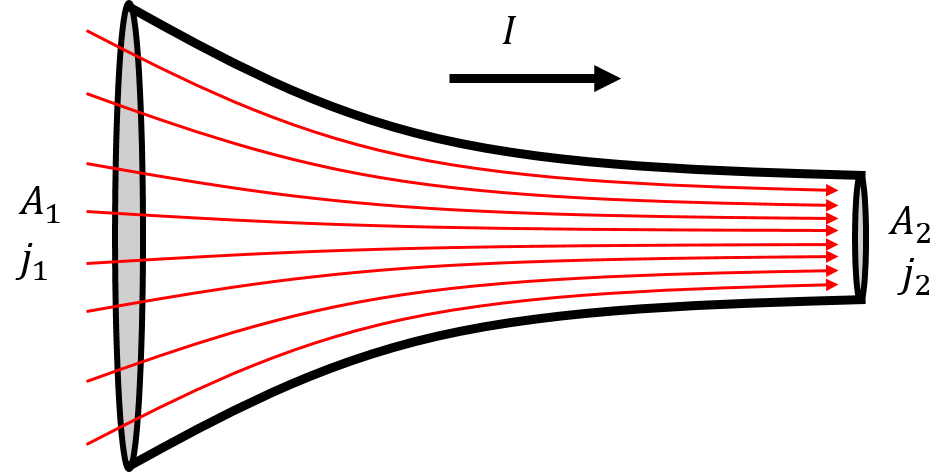
\includegraphics[width=0.5\linewidth]{files/taper-2f6f00dbd2c0235cd9164665ecccfaae.png}
\caption[]{Current flows through a conductor with a cross-section that decreases from $A_1$ to $A_2$.}
\label{fig:current:taper}
\end{figure}

This situation is very similar to the flow of an incompressible fluid. In this case, the number of charges entering the conductor must be equal to the number of charges exiting the conductor during a given amount of time. That is, the total current, $I$, must be the same at both ends, since there is no place in the conductor for charges to accumulate. Since the current must be the same on both ends, we can relate the current densities at each end:
\begin{equation}
j&=\frac{I}{A}\\
\therefore I&=j_1A_1=j_2A_2\\
\therefore \frac{j_2}{j_1}&=\frac{A_1}{A_2}
\end{equation}
and we find that the current density at the exit of the conductor must be higher than at the entrance. This is similar to the continuity equation in the Fluid Mechanics chapter (Section~\ref{sec:fluidmechanics:continuity}), where the current density plays a role analogous to the velocity in the fluids case.
\end{framed}
\end{framed}

\subsubsection{Microscopic model of current}\label{sec:current:micromodel}

Consider a cylindrical conductor of cross-sectional area $A$ and length $L$, as shown in Figure~\ref{fig:current:collisions}. A potential difference, $\Delta V$, is applied across the length of the conductor, so that there is an electric field, $\vec E$, everywhere within the conductor. If the conductor were made of empty space, electrons would enter one end of the conductor, accelerate through the potential difference, and arrive at the other end with a high speed, having gained $e\Delta V$ of kinetic energy. In reality, the conductor is made of matter, and electrons do not accelerate continuously through the whole length of the conductor. Instead, they can only accelerate over a short distance before colliding with an atom in the material (rather, a tightly bound electron in the material), and losing their kinetic energy to the material, before accelerating again. The motion of electrons flowing in a conductor is illustrated in Figure~\ref{fig:current:collisions} and shows electrons moving with a wide range of velocities following the collisions, and only an average motion in the direction anti-parallel to the electric field.

\begin{figure}[!htbp]
\centering
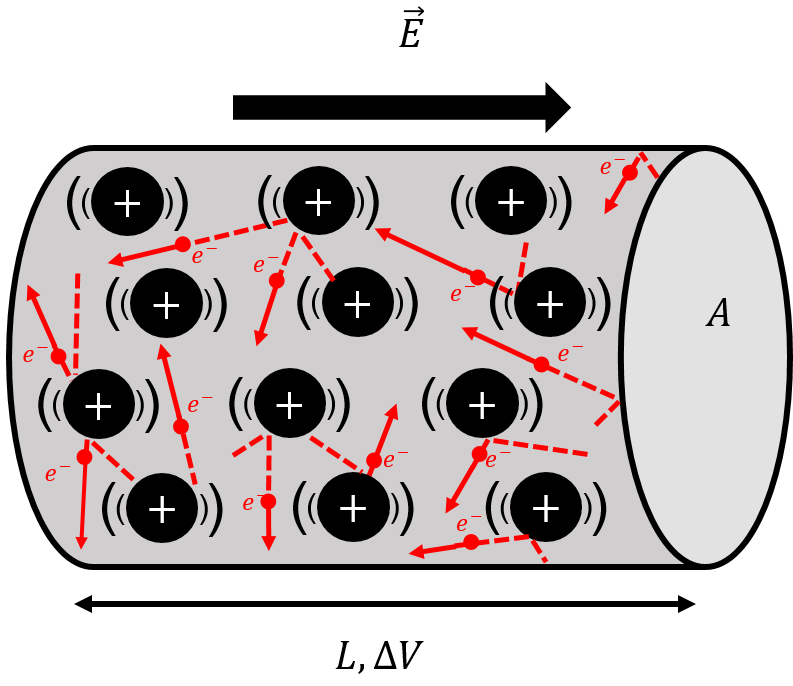
\includegraphics[width=0.4\linewidth]{files/collisions-bb5c391e996427814e4a857ff6bd18f5.png}
\caption[]{Electrons moving inside a conductor only ``drift'' on average in the direction anti-parallel to the electric field. In reality, they constantly collide with atoms in the material, transferring their kinetic energy into thermal energy of the conductor.}
\label{fig:current:collisions}
\end{figure}

Thus, when the electrons arrive at the positive side of the conductor, they have not gained any kinetic energy. Instead, they have lost that kinetic energy to atoms of the conducting material through collisions; those atoms then vibrate which we can measure as an increase in temperature of the material. When current flows through a conductor, that conductor will heat up; this is how the heating elements in your toaster work!

We model the motion of electrons as charges ``drifting'' through the conductor with a velocity $\vec v_d$, the ``drift velocity'', as illustrated in Figure~\ref{fig:current:microcurrent}. In reality, of course, the electrons are only moving on average with the drift velocity, and their instantaneous speed is generally much larger than the drift velocity and can be in any direction, as illustrated in Figure~\ref{fig:current:collisions}.

\begin{figure}[!htbp]
\centering
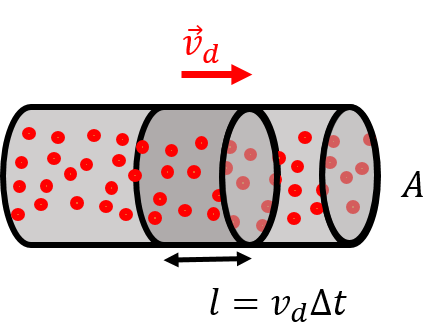
\includegraphics[width=0.4\linewidth]{files/microcurrent-f26d3b3d3edf9ea7da4f38af7b2acf72.png}
\caption[]{A section of electrons of length $l$ drifting through a conductor of cross-sectional area, $A$.}
\label{fig:current:microcurrent}
\end{figure}

In a conducting material, each atom will generally have one ``free'' electron that is loosely bound and able to easily move through the material. The number of free electrons available for conduction per unit volume, $n$, will depend on properties of the material (its density, how many electrons per atom are available, etc). Consider the motion of the conduction electrons present in a section of length $l$ of a conductor, as illustrated in Figure~\ref{fig:current:microcurrent}. The amount of charge, $\Delta Q$, contained in a section of the conductor with length $l$ is given by:
\begin{equation}
\Delta Q= -e n Al
\end{equation}
where $Al$ is the volume of that section of the conductor, and $e$ is the magnitude of the charge of the electron. The negative sign is to indicate that the charges are negative (they are electrons). That charge will take an amount of time, $\Delta t$, to flow through a given plane of the conductor, so that we can relate the length of the section, $l$, to the drift speed and $\Delta t$:
\begin{equation}
l&=v_d\Delta t
\end{equation}
Thus, the current that flows through a cross-section of the conductor is given by:
\begin{equation}
I=\frac{\Delta Q}{\Delta t}=\frac{-e n Al}{\Delta t}=-enAv_d
\end{equation}
\begin{equation}
\therefore\;\boxed{I=-enAv_d},
\end{equation}
which allows us to connect a macroscopic quantity, current, to the microscopic description of moving charges. Note that the negative sign reflects the fact that the current (of positive charges) is in the opposite direction from the drift velocity of the (negative) electrons. The current density is directly related to the microscopic quantities, since it does not depend on the (macroscopic) cross-sectional area, $A$, of the conductor:
\begin{equation}
\vec j&=\frac{I}{A}\hat E = -en\vec v_d
\end{equation}
\begin{equation}
\therefore\; \boxed{\vec j = -en\vec v_d}
\end{equation}
where, again, the negative sign indicates that the current density is in the opposite direction from the actual drift velocity of the electrons, which itself is anti-parallel to the electric field.

\begin{framed}
\textbf{Example 18.2}\\
A current of $1 {\rm A}$ is measured in a copper wire with a diameter of $1 {\rm mm}$. What is the drift velocity of the electrons? Assume that each atom of copper provides one ``free electron'' for conduction.

\begin{framed}
\textbf{Solution}\\
In order to determine the drift velocity of electrons, we need to know the density of free electrons in copper. To do this, we need to determine how many copper atoms there are per unit volume. The density of copper is $\rho=8.92e3 {\rm kg/m^3}$ and the atomic mass unit of copper is $63.5 {\rm amu}$ ($1 {\rm mole}$ of copper weighs $63.5 {\rm g}$). The number of copper atoms per unit volume is thus:
\begin{equation}
n=\frac{(6.022e23 {\rm mole^{-1}})(8.92e3 {\rm kg/m^3})}{(63.5e-3 {\rm kg/mole})}=8.46e28 {\rm m^{-3}}
\end{equation}
Since each copper atom contributes one free electron, this is the same as the density of free electrons. From this, we easily obtain the drift velocity from the current:
\begin{equation}
v_d&=\frac{j}{en}=\frac{I}{Aen}=\frac{(1 {\rm A})}{\pi(0.0005 {\rm m})^2(1.6e-19 {\rm C})(8.46e28 {\rm m^{-3}})}\\
&=9.4e-5 {\rm m/s}\sim0.1 {\rm mm/s}
\end{equation}
The drift velocity is thus very slow, less than one millimetre per second. Note that a $1 {\rm mm}$ diameter copper wire would not actually be able to sustain such a high current density without damage.
\end{framed}
\end{framed}

\begin{framed}
\textbf{Josh's Thoughts}\\
There are a few types of velocities which can be easily confused when discussing current: Fermi velocity, drift velocity, and the velocity at which a circuit is ``completed''.

Understanding the Fermi velocity requires quantum mechanics and is beyond the scope of this textbook. However, the Fermi velocity is representative of the actual velocity of electrons in a conducting material, mostly due to their thermal energy. In a good conductor, these speed are roughly 1/200 the speed of light.

While electrons do move at their Fermi velocity in a conductor, they do not move in a uniform path through the conductor towards the end of the circuit. Most of an electron's movement in a wire is chaotic, but in a DC circuit, the electrons have a drift velocity through the conductor. This drift velocity is defined as the net velocity of electrons in a conductor, and is caused by the applied electric field which has a small amount of influence on the direction of the quickly moving electron's motion. The drift velocity of electrons is very slow, often having a magnitude as small as tens of microns per second.

When comparing drift velocity to Fermi speed, imagine yourself standing inside of a large horizontal cylinder, which will represent the conductor in this analogy. The interior of this cylinder is lined with cannons that shoot rubber balls in all directions, which will be the electrons moving at their Fermi velocity. Now, imagine that you are attempting to move these high-speed rubber balls from one end of the cylinder to the other by blowing a hair dryer in that direction, which is the electric field inducing a drift velocity.

Now that we understand the quantum chaos that occurs in a conductor, you may be thinking to yourself, ``why does the light bulb turn on so quickly after I flick the light switch?''. This is a reasonable thought, because we have only covered the motion of single particles in a conductor. When an electron moves very slightly (at its drift velocity), it will push other electrons in the conductor forward, causing a chain reaction of electrons pushing one another forward. This movement causes electrons to flow through the circuit, much like how water flows through a pipe. The velocity at which a light bulb turns on after the flicking of a switch is theoretically the speed of light, but short delays caused by irregularities in the way electrons bump into one another causes the velocity to be roughly 50 to 99 percent of the speed of light.
\end{framed}

\subsubsection{Ohm's Law}

In the previous section, we developed a microscopic model of charges moving in a conductor, but did not describe how this motion is affected by the electric field in the conductor (or equivalently, the potential difference across the conductor). ``Ohm's Law'' states that the current density, $\vec j$, at some position in the conductor is proportional to the electric field, $\vec E$, at that same position in the conductor:
\begin{equation}
\vec j \propto \vec E
\end{equation}
\begin{equation}
\boxed{\vec j = \sigma \vec E}
\end{equation}
where we have introduced the ``conductivity'', $\sigma$, as the constant of proportionality. Conductivity is a property of the material from which the conductor is made, and is a measure of how large a current density (and by extension, current) there will be in material given a certain electric field. Materials with a high conductivity are said to be good conductors, as a large current will result from a small electric field. Gold and copper are examples of materials with a high conductivity.

\begin{framed}
\textbf{Checkpoint}\\
What is the conductivity of an ideal insulator?

\begin{enumerate}
\item 0
\item Roughly 1
\item Infinite
\end{enumerate}

\begin{framed}
\textbf{Answer}\\
\begin{enumerate}
\item
\end{enumerate}
\end{framed}
\end{framed}

\paragraph{Resistivity}

For convenience, one often describes how well a material conducts charges using the ``resistivity'', $\rho$, which is simply defined as the inverse of conductivity:
\begin{equation}
\rho = \frac{1}{\sigma}
\end{equation}
Materials with a high resistivity are poor conductors; they tend to ``resist'' the formation of a current when an electric field is applied. Insulators have high resistivity.

The resistivity of most (but not all) materials has been observed to increase linearly with the temperature of the material. One can picture that, as atoms in the material vibrate more, it is more difficult for electrons to conduct through the material as they will interact with more atoms. The resistivity, $\rho$, at a certain temperature, $T$, is usually modelled as follows:
\begin{equation}
\rho(T)=\rho_0\left[ 1 + \alpha (T-T_0)\right]
\end{equation}
where $\rho_0$ is a ``reference resistivity'' measured at a ``reference temperature'', $T_0$ (usually $20 {\rm \degree C}$). The constant $\alpha$ is the ``temperature coefficient'' of the material. The temperature dependence of the resistivity is illustrated in Figure~\ref{fig:current:resistivity}.

\begin{figure}[!htbp]
\centering
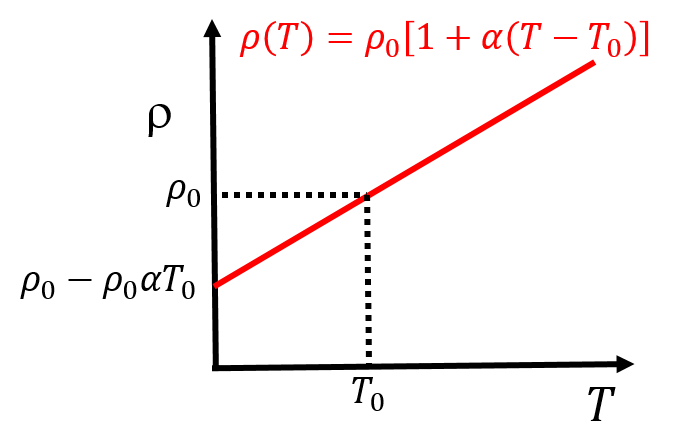
\includegraphics[width=0.4\linewidth]{files/resistivity-c7aafb366a6b3b1ed6353f119b1917bd.png}
\caption[]{A linear model of resistivity can be used for most conductors over a large range of temperatures.}
\label{fig:current:resistivity}
\end{figure}

This ``linear model'' (since resistivity increases linearly with temperature) is empirically found to be valid for many materials over a large range of temperatures, although it is not expected to hold at extreme temperatures (either very low or very high). Furthermore, for semi-conducting materials (such as silicon and germanium), resistivity is found to decrease as a function of temperature.

\begin{framed}
\textbf{Checkpoint}\\
What is the slope of the resistivity vs temperature as shown in Figure~\ref{fig:current:resistivity}?

\begin{enumerate}
\item $\alpha$.
\item $\rho_0 \alpha T$.
\item $\rho_0 T$.
\item $\rho_0 \alpha$.
\end{enumerate}

\begin{framed}
\textbf{Answer}\\
\begin{enumerate}[resume]
\item
\end{enumerate}
\end{framed}
\end{framed}

Table~\ref{tab:current:materials} shows a list of common materials and their conductivity, resistivity, and temperature coefficients (defined at a reference temperature $T_0=20 {\rm \degree C}$).

\begin{table}
\centering
\caption[]{Resistivity, free electron density and temperature coefficients of common materials. All properties are listed for a reference temperature of $20 {\rm \degree}C$.}
\label{tab:current:materials}
\begin{tabular}{p{\dimexpr 0.250\linewidth-2\tabcolsep}p{\dimexpr 0.250\linewidth-2\tabcolsep}p{\dimexpr 0.250\linewidth-2\tabcolsep}p{\dimexpr 0.250\linewidth-2\tabcolsep}}
\toprule
\textbf{Material} & \textbf{Resistivity} ${\rm \left[{\Omega\cdot m}\right]}$ & \textbf{Temperature coefficient} ${\rm \left[{\degree C^{ -1}}\right]}$ & \textbf{Free electron density}${\rm \left[{m^{ -3}}\right]}$ \\
\hline
Silver & $1.59\times 10^{ -8}$ & 0.0038 & $5.86\times 10^{28}$ \\
Copper & $1.68\times 10^{ -8}$ & 0.0040 & $8.46\times 10^{28}$ \\
Gold & $2.44\times 10^{ -8}$ & 0.0034 & $5.90\times 10^{28}$ \\
Aluminum & $2.74\times 10^{ -8}$ & 0.0039 & $18.1\times 10^{28}$ \\
Iron & $9.70\times 10^{ -8}$ & 0.0050 & $17.0\times 10^{28}$ \\
Silicon & $0.1 -1000$ & -0.0750 & 0 \\
Rubber & $(1 -100)\times 10^{13}$ & 0 & 0 \\
Quartz & $7.5\times 10^{17}$ & 0 & 0 \\
\bottomrule
\end{tabular}
\end{table}

\subsubsection{Resistors}

A conductor with current going through it (or current that could go through it) is generally called a ``resistor'' to emphasize that charges will experience resistance as they travel through the conductor (as they collide with atoms). In this section, we describe resistors, how to combine them, and how to model the heat that is generated when charges collide with the atoms in the resistor.

\paragraph{Resistance}

Consider a resistor with length $L$ and cross-sectional area $A$, made out of a material with resistivity $\rho$, as illustrated in Figure~\ref{fig:current:resistor}.

\begin{figure}[!htbp]
\centering
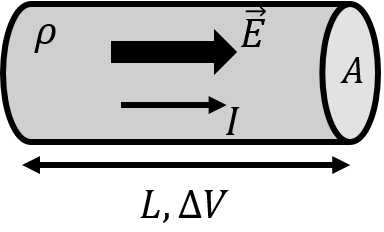
\includegraphics[width=0.3\linewidth]{files/resistor-19789ed5da193d469511eec922645ce0.png}
\caption[]{A simple resistor of length, $L$, cross-sectional area, $A$, made from a materials with resistivity, $\rho$. A potential difference, $\Delta V$, is applied across the resistor, leading to an electric field and current in the resistor.}
\label{fig:current:resistor}
\end{figure}

A potential difference, $\Delta V$, is applied across the length of the resistor, resulting in an electric field, $\vec E$, within its volume. To good approximation, one can model the two ends of the conductor as parallel plates, so that the magnitude of the electric field throughout the conductor is constant in magnitude and direction and has strength given by:
\begin{equation}
E=\frac{\Delta V}{L}
\end{equation}
Combining this with Ohm's Law, we have:
\begin{equation}
j&=\sigma E\\
\therefore j&=\sigma\frac{\Delta V}{L}\\
\end{equation}
Since the current density is a microscopic quantity, we can replace it with the current, $I$, a macroscopic quantity, for the conductor of cross-sectional area $A$, to find:
\begin{equation}
j&=\frac{I}{A}\\
\therefore I&=jA=\sigma\frac{\Delta V}{L}A
\end{equation}
This last equation is often written by isolating the potential difference:
\begin{equation}
\boxed{\Delta V = \rho \frac{L}{A} I}
\end{equation}
where we replaced the inverse of the conductivity with the resistivity. This last equation is the equivalent of Ohm's Law, but written for a (macroscopic) resistor of length $L$, cross-sectional area $A$, and made of a material with resistivity, $\rho$. Written in this way, Ohm's Law is a statement that the \textbf{current through a resistor is proportional to the voltage applied across it}. The constant of proportionality, $R$, is called the ``resistance'':
\begin{equation}
\boxed{\Delta V = RI}
\end{equation}
This last equation is often called ``Ohm's Law'', even if, technically, Ohm's Law is the relation between current density and electric field. A resistor is a macroscopic object whose ``resistance'' can be characterized by a single value, $R$, its resistance. The resistance of a resistor can be determined from its macroscopic properties (length and cross-sectional area) and from the material from which it is made (with a given resistivity):
\begin{equation}
\boxed{R = \rho \frac{L}{A} }
\end{equation}
The (derived) S.I. unit of resistance is the ``Ohm'', (${\rm\Omega}$).

\begin{framed}
\textbf{Olivia's Thoughts}\\
Resistivity versus Resistance: Both resistance and resistivity tell us how strongly a material or conductor opposes the flow of current. The difference is that the resistivity is a fundamental property of a material (and is microscopic), whereas resistance depends on the size and shape of the conductor, \textit{as well as} the resistivity (and is macroscopic). It is tempting to think about resistivity as the ``resistance density'', because it is similar to the concepts of mass density and charge density. However, we have to be careful because resistivity is not resistance per unit volume ($\rho \neq R/(A\cdot L)$), and is instead related to resistance by $\rho=R\cdot (A/L)$.
\end{framed}

\begin{framed}
\textbf{Checkpoint}\\
What are the SI units of conductivity?

\begin{enumerate}
\item ${\rm \frac{\Omega}{C}}$.
\item ${\rm \frac{1}{\Omega m}}$.
\item ${\rm \frac{N^2 \Omega}{C}}$.
\item ${\rm \frac{C}{s}}$.
\end{enumerate}

\begin{framed}
\textbf{Answer}\\
\begin{enumerate}[resume]
\item
\end{enumerate}
\end{framed}
\end{framed}

The model to describe the resistance of a conductor to the flow of electric current under a fixed potential difference, $\Delta V$, is identical to the model that we derived in Section~\ref{sec:fluidmechanics:poiseuille} to describe the Poiseuille flow, $Q$, of an viscous incompressible fluid in a pipe with resistance, $R$, under a pressure difference, $\Delta P$:
\begin{equation}
\Delta P = RQ
\end{equation}
Thus, one can think of electric current by analogy to the incompressible flow of a viscous fluid through a pipe. If the pipe is longer, it opposes more resistance to the flow of liquid, just as a longer resistor has a larger resistance to current. A pipe with a larger cross-sectional area has less resistance to the flow of liquid, just as a resistor with a larger cross sectional area, $A$, has a lower resistance.

\paragraph{Combining resistors}

Resistors are the most common component in circuits, and we show below how to model the equivalent resistance of two resistors that are combined in ``parallel'' or in ``series''.

Figure~\ref{fig:current:series} shows two resistors, $R_1$ and $R_2$, connected in ``series'', to form an an effective resistor with resistance $R_{eff}$. A potential difference, $\Delta V$, is applied across the combination of resistors.

\begin{figure}[!htbp]
\centering
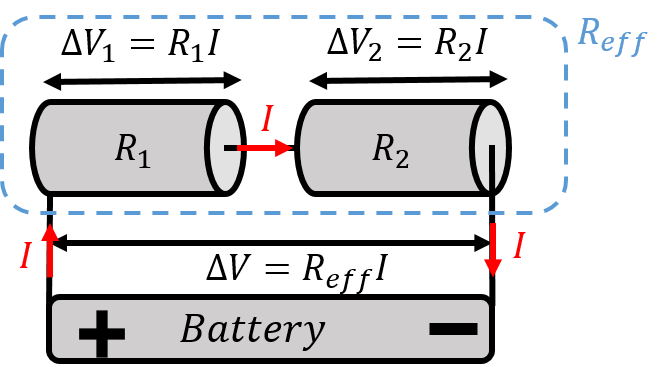
\includegraphics[width=0.45\linewidth]{files/series-89b8fcc9f34dfbdec77541ffdf727f64.png}
\caption[]{When two resistors are connected in series, the same current flows through each resistor.}
\label{fig:current:series}
\end{figure}

By analogy with fluid mechanics, the charges that enter the first resistor, $R_1$, must exit the resistor at the same rate, and then cross the second resistor, $R_2$. In other words, what comes into $R_1$ must come back out of $R_2$, since there is no place for the charges to go. This is the electrical equivalent of ``continuity'' in fluid mechanics. \textbf{When resistors are combined in series, both resistors will have the same current, $I$, through them}.

Ohm's Law (the macroscopic version), must also be true for each resistor:
\begin{equation}
\Delta V_1 &= R_1I\\
\Delta V_2 &= R_2I
\end{equation}
where $\Delta V_1$ and $\Delta V_2$ are the potential differences across each resistor. $\Delta V_1$ and $\Delta V_2$ must sum to $\Delta V$:
\begin{equation}
\Delta V_1 + \Delta V_2=\Delta V
\end{equation}
since the potential energy (per unit charge) that is lost in each resistor must equal to the total potential energy (per unit charge) that is made available by the battery. Combining this last equation with Ohm's Law for each resistor, we can model the series combination of resistors as having an ``effective resistance'', $R_{eff}$, given by:
\begin{equation}
\Delta V = \Delta V_1 + \Delta V_2=R_1I+R_2I=(R_1+R_2)I=R_{eff}I
\end{equation}
\begin{equation}
 \boxed{R_{eff}=R_1+R_2}\quad \text{(Series resistors)}
\end{equation}
It makes sense that the equivalent resistance is found by summing the two resistors when they are in series. If the two resistors are made of the same material and have the same cross-sectional area, combining them in series is equivalent to fabricating a longer resistor with the two lengths added together. The result is easily extended to any number of resistors:
\begin{equation}
R_{eff}&=R_1+R_2+R_2+\dots
\end{equation}

\begin{framed}
\textbf{Olivia's Thoughts}\\
The comparison to fluid mechanics can very useful. In the left panel of Figure~\ref{fig:current:waterseries}, I've shown what the series circuit from Figure~\ref{fig:current:series} would look like in the fluid mechanics analogy. Here, I have replaced the current with the fluid flow, $Q$, and the voltage with the pressure differential, $\Delta P$. The resistors are now narrow portions of the pipe, with resistances $R_1$ and $R_2$. There are a couple things we can see from this:

\begin{enumerate}
\item The flow is the same at every point along the circuit, because there is only one path the water can take, and there is no build up of water at any point.
\item The effective resistance is the sum of $R_1$ and $R_2$, because the resistance from the two narrow sections is equivalent to the resistance of one long narrow section, as displayed in the right panel of Figure~\ref{fig:current:waterseries}.
\end{enumerate}

\begin{figure}[!htbp]
\centering
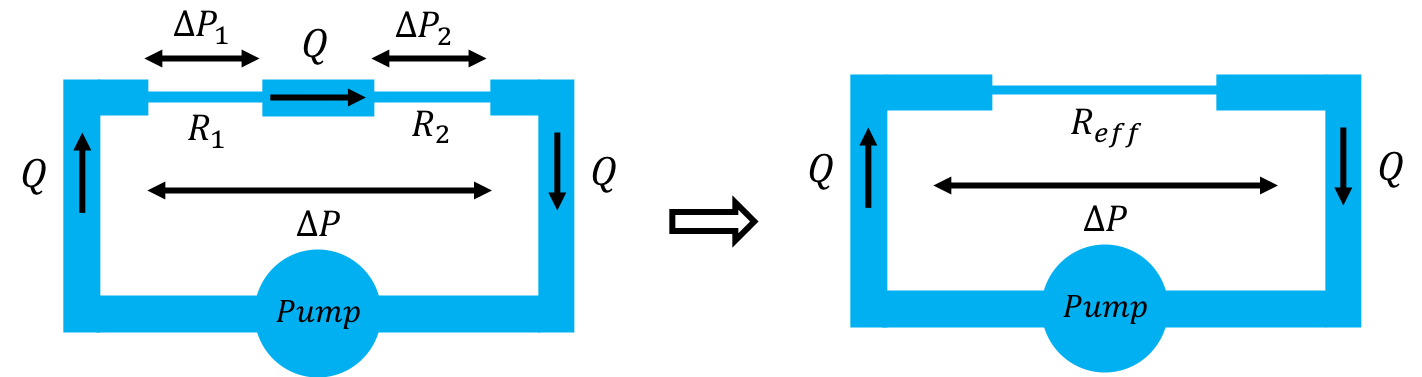
\includegraphics[width=0.7\linewidth]{files/waterseries-7eef2efa94ac989eef10ef8de3522596.png}
\caption[]{Left panel: What a series circuit would look like in the context of fluid mechanics. Right panel: The two resistors can be thought of as a single resistor with effective resistance $R_{eff}=R_1+R_2$.}
\label{fig:current:waterseries}
\end{figure}
\end{framed}

Figure~\ref{fig:current:parallel} shows two resistors, with resistances $R_1$ and $R_2$, combined in parallel to form an effective resistor with resistance, $R_{eff}$. A potential difference, $\Delta V$, is applied across the combination of resistors. \textbf{When resistors are combined in parallel, both resistors have the same potential difference across them}.

\begin{figure}[!htbp]
\centering
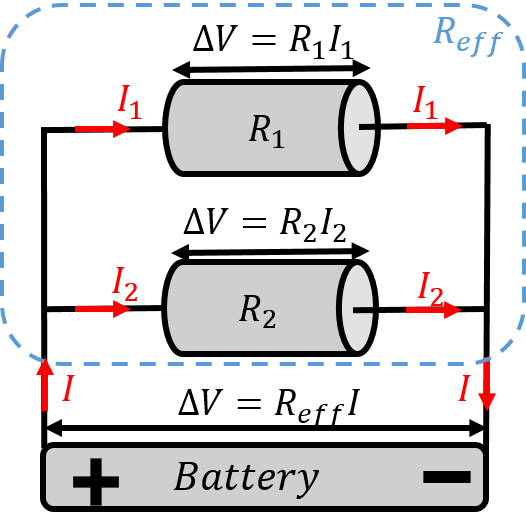
\includegraphics[width=0.4\linewidth]{files/parallel-d0205dcfa0a04a47e822005ba14cdb89.png}
\caption[]{When two resistors are connected in parallel, the same voltage is applied across each resistor.}
\label{fig:current:parallel}
\end{figure}

Applying Ohm's Law to each resistor, we find that they each have difference currents going through them:
\begin{equation}
I_1&=\frac{\Delta V}{R_1}\\
I_2&=\frac{\Delta V}{R_2}
\end{equation}

The total current, $I$, that enters the combination of resistors, must also exit the combination of resistors (continuity), so that the total current, $I$, is the sum of the current through each resistor:
\begin{equation}
I=I_1+I_2
\end{equation}
Combining this with Ohm's Law, we find:
\begin{equation}
I&=I_1+I_2=\frac{\Delta V}{R_1}+\frac{\Delta V}{R_2}=\left( \frac{1}{R_1}+\frac{1}{R_2} \right)\Delta V\\
\therefore \Delta V &= \frac{1}{\frac{1}{R_1}+\frac{1}{R_2}}I
\end{equation}
Thus, the effective resistance, $R_{eff}$, of two resistors connected in parallel is given by:
\begin{equation}
\boxed{R_{eff}=\frac{1}{\frac{1}{R_1}+\frac{1}{R_2}}=\frac{R_1R_2}{R_1+R_2}}\quad \text{(Parallel resistors)}
\end{equation}
where the two forms that are given are equivalent. The effective resistance of two resistors in parallel is smaller than the resistance of either resistor. This makes sense, because combining resistors in parallel is analogous to fabricating a single resistance with a larger cross-sectional area, allowing for ``more space'' for the charges to flow. Again, this result is easily extended for more than two resistors:
\begin{equation}
R_{eff}=\frac{1}{\frac{1}{R_1}+\frac{1}{R_2}+\frac{1}{R_3}+\dots}
\end{equation}

\begin{framed}
\textbf{Olivia's Thoughts}\\
Once again, we can use the comparison to fluid mechanics. The left panel of Figure~\ref{fig:current:waterparallel} shows what the parallel circuit in Figure~\ref{fig:current:parallel} would look like in the fluid mechanics analogy. There are a couple things we can take from this:

\begin{enumerate}
\item Now, there are two paths that the water can take, so the flow through $R_1$ will not necessarily be the same as that though $R_2$. However, since there are only two paths to take, the total flow must be equal to the sum of the flow through each resistor (i.e. $Q=Q_1+Q_2$).
\item The effective resistance is lower than the individual resistances $R_1$ and $R_2$. The two narrow resistors are equivalent to one wider resistor, as in Figure~\ref{fig:current:waterparallel}.
\end{enumerate}

\begin{figure}[!htbp]
\centering
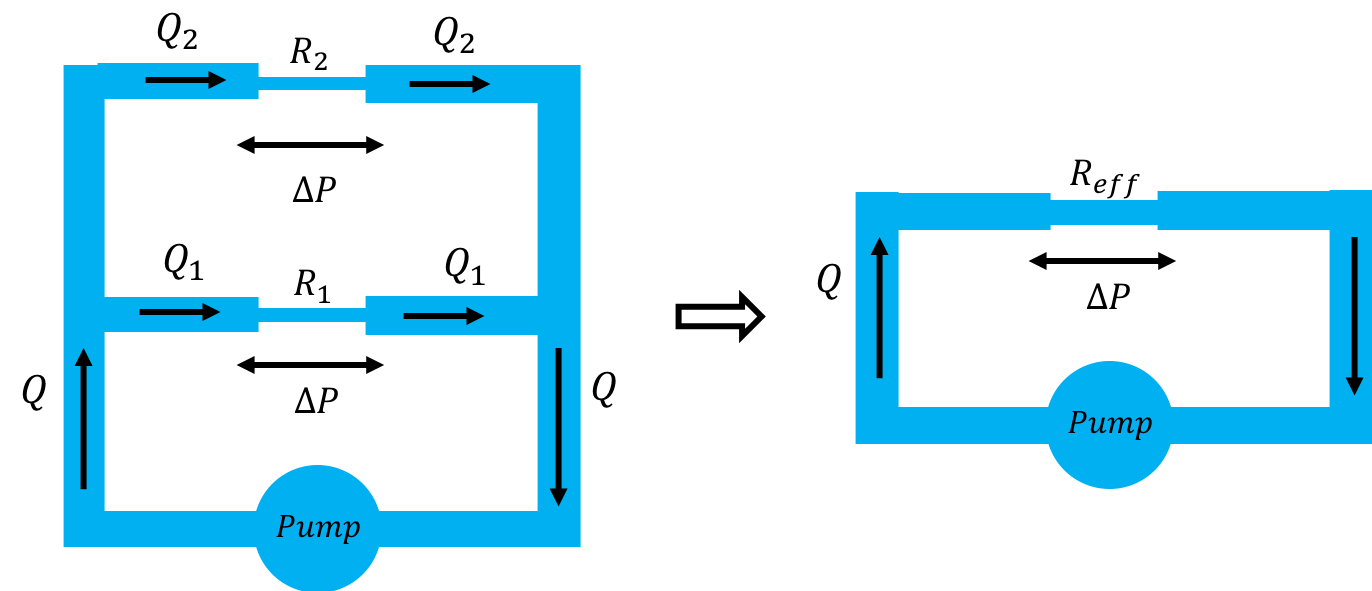
\includegraphics[width=0.7\linewidth]{files/waterparallel-185622bb6a9f5dca18b789894c44d66f.png}
\caption[]{Left panel: What a parallel circuit would look like in the context of fluid mechanics. Right panel: The two resistors can be thought of as a single, wide resistor with effective resistance $R_{eff}=(1/R_1)+(1/R_2)$.}
\label{fig:current:waterparallel}
\end{figure}
\end{framed}

\begin{framed}
\textbf{Example 18.3}\\
A $R_2=2 {\rm \Omega}$ resistor is placed in parallel with a $R_3=3 {\rm \Omega}$ resistor and the combination is placed in series with a $R_1=1 {\rm \Omega}$ resistor, as shown in Figure~\ref{fig:current:3resistors}. What is the effective resistance of this combination?

\begin{framed}
\textbf{Solution}\\
\begin{figure}[!htbp]
\centering
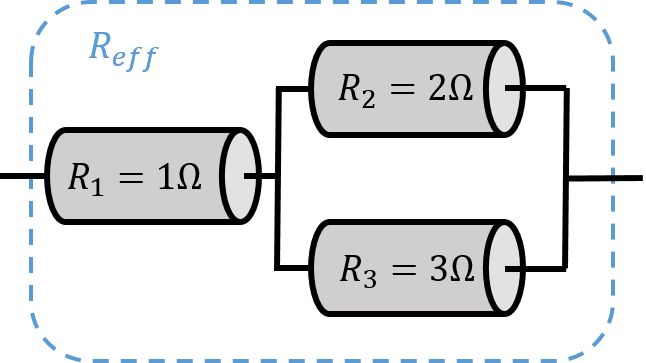
\includegraphics[width=0.4\linewidth]{files/3resistors-5f2efd2bb3dd619606b3f808340d707b.png}
\caption[]{A combination of three resistors.}
\label{fig:current:3resistors}
\end{figure}

In order to determine the effective resistance of the combination, we can first combine the parallel resistors $R_2$ and $R_3$ into an effective resistor, $R'$, which we can then combine in series with the resistor $R_1$, to obtain the effective resistance of the three resistors. First, combining the parallel resistors, $R_2$ and $R_3$, we find:
\begin{equation}
R'=\frac{R_2R_3}{R_2+R_3}=\frac{6}{5}{\rm\Omega}
\end{equation}
We can then combine this in series with $R_1$, to obtain the total effective resistance of the combination of three resistors:
\begin{equation}
R_{eff}=R_1+R'=\frac{11}{5}{\rm\Omega}
\end{equation}
**Discussion: **In this example, we showed how to determine the effective resistance of a combination of series and parallel resistors. We can determine the effective resistance of complex combinations of resistors in the same manner, by first combining subsets of resistors and then including those with other resistors.
\end{framed}
\end{framed}

\paragraph{Electrical power dissipated in resistors}

As we discussed in Section~\ref{sec:current:micromodel}, charges that move through a resistor do not gain kinetic energy. Instead, the electric potential energy available from the voltage applied across the resistor is converted into heat, as a result of charges colliding with atoms in the material. The net potential energy, $\Delta U$, available to a single charge, $q$, is given by:
\begin{equation}
\Delta U=q\Delta V
\end{equation}
If there are many charges going through the resistor, the rate, $P$, at which they will dissipate energy in the resistor is given by:
\begin{equation}
P&=\frac{d}{dt}\Delta U=\frac{d}{dt}q\Delta V=I\Delta V\\
\therefore P&=I\Delta V
\end{equation}
where we recognized that $dq/dt=I$ is the definition of current. $P$ corresponds to the rate at which energy is dissipated in the resistor, and has dimensions of power. Combining this with Ohm's Law, the power that is dissipated in a resistor can be written in different ways:
\begin{equation}
\boxed{P=I \Delta V=\frac{(\Delta V)^2}{R}=I^2R}
\end{equation}
\begin{framed}
\textbf{Example 18.4}\\
A hair-dryer is rated as consuming $1500 {\rm W}$ when connected to an outlet with a $120 {\rm V}$ potential difference. What is the resistance of the hair-dryer, and how much current goes through it when it is running?

\begin{framed}
\textbf{Solution}\\
Since the power of the hair-dryer and the potential difference across it are known, we can easily determine its resistance:
\begin{equation}
P&=\frac{(\Delta V)^2}{R}\\
\therefore R&=\frac{(\Delta V)^2}{P}=\frac{(120 {\rm V})^2}{(1500 {\rm W})}=9.6 {\rm \Omega}
\end{equation}
Similarly, we can determine the current through the hair dryer:
\begin{equation}
P&=I\Delta V\\
\therefore I &=\frac{P}{\Delta V}=\frac{(1500 {\rm W})}{(120 {\rm V})}=12.5 {\rm A}
\end{equation}
**Discussion: **Most household appliances are rated by the electrical power that they consume. This rating assumes that the appliance will be connected to a fixed potential difference ($120 {\rm V}$ in North America), so it is  straightforward to determine the current that they will draw. This is important because the current that is drawn by the appliance has to go through the wiring in the house, and if the current is too large, the wiring (which has resistance) will heat up ($P=I^2R$) which could result in an electrical fire. Circuits in a house have safety devices (fuses or breakers) that are designed to interrupt the circuit if the current is too large.
\end{framed}
\end{framed}

One can rate a power supply, such as a battery, by the amount of power that it can deliver. Power supplies are usually designed to supply a fixed potential difference; for example, a $9 {\rm V}$ battery supplies a constant voltage of $9 {\rm V}$. If a small resistor is connected across the terminals of the battery, a large current, $I$, will flow through the resistor. In principle, the current through the resistor will be given by Ohm's Law, $I=\Delta V/R$. However, by reducing the resistance, the current will increase, and the power dissipated by the resistor, $P=I\Delta V$, would increase indefinitely. Obviously, this is not possible, as it requires the battery to supply energy at the same, ever increasing rate. In practice, as the resistance is decreased, the current through the resistor will only increase until $I \Delta V$ is equal to the maximal power that can be dissipated by the battery. As the resistance across the battery is further decreased, the voltage across the battery will start to decrease as well, so that the power dissipated in the resistor, $I \Delta V$, does not exceed the power that the battery could possibly supply.

\paragraph{Superconductors}

Superconductors are materials that, under certain conditions, have zero resistivity. A resistor made from a superconducting material will thus have zero resistance. It is beyond the scope of this textbook to describe how superconductivity arises in materials, however, it is worth knowing that these exist. Typically, superconductivity arises in materials when they are cooled to temperatures close to absolute zero, although some materials exhibit superconductivity at much higher temperatures ($\sim140 {\rm K}$ or $\sim -130 {\rm \degree C}$). Superconducting materials are often used when one needs a large electric current, such as in a powerful electro-magnet. By having no resistance, a large current can be sustained without dissipating any power.

\subsubsection{Alternating voltages and currents}

So far, we have modelled how current propagates through a resistor under a constant potential difference, $\Delta V$. This is called ``direct current'' (DC) as the charges move in a constant direction through the resistor. Batteries supply fixed voltages, and circuits with batteries will almost always have DC current. The voltage that is supplied between two of the sockets in a household electrical outlet is ``alternating'', and leads to ``alternating current'' (AC), where charges move back and forth, with no net displacement.

The potential difference across a household outlet varies sinusoidally:
\begin{equation}
\Delta V (t) = \Delta V_0 \sin(\omega t)
\end{equation}
where $\Delta V_0$ is the maximal amplitude of the voltage ($120 {\rm V}$ in North America, $220 {\rm V}$ in Europe), and $\omega = 2\pi f$ is the angular frequency of the voltage ($f=60 {\rm Hz}$ in North America, $f=50 {\rm Hz}$ in Europe). When a resistor with resistance $R$ is connected to an AC voltage, the resulting current, given by Ohm's Law, is also alternating:
\begin{equation}
I(t)=\frac{\Delta V(t)}{R}=\frac{\Delta V_0}{R}\sin(\omega t)=I_0\sin(\omega t)
\end{equation}
On average, the alternating current through a resistor is zero. However, this does not mean that zero  energy is dissipated, since the electrons in the resistor will still collide with atoms as they oscillate back and forth. We can define the average power, $\bar P$, that is dissipated in the resistor as the  power that is dissipated over one oscillation cycle (with period, $T$). To obtain the latter, we calculate the total energy, $E$, dissipated in the resistor over one cycle so that the power is simply given by $E/T$. We divide the interval of time, $T$, into infinitesimally small intervals, $dt$, so that the infinitesimal energy, $dE$, dissipated in an infinitesimal time, $dt$, is given by:
\begin{equation}
dE=P(t) dt
\end{equation}
The total energy dissipated in one period is then given by:
\begin{equation}
E=\int dE = \int_0^T P(t)dt
\end{equation}
so that the power dissipated in one cycle is given by:
\begin{equation}
\bar P=\frac{E}{T}=\frac{1}{T}\int_0^T P(t)dt
\end{equation}
The instantaneous power, $P(t)$, can be described in terms of the instantaneous current, $P(t)=I^2(t)R$, so that the average power can be written as:
\begin{equation}
\bar P = \frac{1}{T}\int_0^TP(t)dt=\frac{1}{T}\int_0^TI(t)^2Rdt=RI_0^2\frac{1}{T}\int_0^T\sin^2(\omega t)dt=\frac{1}{2}RI_0^2
\end{equation}
where we used the fact that $T=\frac{2\pi}{\omega}$ to evaluate the integral. In order to make the formula similar to the DC equivalent (without the additional factor of $1/2$), we can define the ``root mean square'' current, $I_{rms}$, as an average current, from which we can calculate the average power that is dissipated in a resistor:
\begin{equation}
I_{rms}&=\frac{I_0}{\sqrt 2}\\
\therefore\bar P&=I_{rms}^2R
\end{equation}
Similarly, one can define the ``root mean square'' voltage, $\Delta V_{rms}$, so that the average power dissipated with an alternating current can be written in the same form as for the DC case:
\begin{equation}
V_{rms}&=\frac{\Delta V_0}{\sqrt 2}\\
\therefore\bar P&=I_{rms}^2R =\frac{\Delta V_{rms}^2}{R}=I_{rms}\Delta V_{rms}
\end{equation}

\subsubsection{Electrical safety}

The models that we have developed to describe current can inform us on ways to avoid being injured by electricity in our common lives. The two main hazards associated with electricity are fire and electrocution. Typically, an electrical fire is the result of a large current going through a resistor, as the power dissipated in a resistor is proportional the square of the current through that resistor. If you connect an appliance that draws a large current to your outlets, the wires in your house (i.e. resistors) could heat up enough to cause a fire (e.g. by heating up insulation that is close by). This danger is primarily mitigated by using ``fuses'' or ``circuit breakers'' that will interrupt the circuit if the current is too large. A fuse is a simple device with a thin wire (high resistance) that will melt and break if too much current goes through it (which is designed to happen long before the wires in your house start to overheat). A circuit breaker is a resettable switch that opens under a large current. Modern houses do not use fuses any more, since they have to be replaced every time they are ``blown''.

Electrocution is a form of injury that is the result of a current crossing the body; we can think of the body as a resistor connected between the terminals of a battery. Injuries can be caused simply by burns (tissue destroyed), or by muscles contracting involuntarily due to the current. For example, one's muscles may contract in such a way that the person cannot let go of the source of current. If a current of more than about $80 {\rm mA}$ passes through the mid section of a person, enough current could go through the heart so that it starts to beat very irregularly (``ventricular fibrillation'') which can lead to death since blood stops flowing normally. A very large current can cause the heart to simply stop beating, which could sometimes be less dangerous than ventricular fibrillation (if for a short period of time, and of course, the burns will be more severe from a larger current). A ``defibrillator'' is designed to provide such a high current that the heart stops briefly, with the hope that when it starts back, the beats will be regular. This can be used in cases of ventricular fibrillation (caused by electrocution or other). One often hears that ``it's current that kills'', which is a statement that being electrocuted by a certain voltage is not a good measure of the resulting injury, since the current will depend on the resistance of the person's body.

The amount of current that will go through a person will depend on the resistance of the person's body. Internal tissues and organs are typically quite conductive and have low resistance. The outer layer of the skin, on the other hand, has a high resistance when dry and helps to limit the current that can go through the body. The resistance of dry skin is usually considerably above $1e4 {\rm \Omega}$, while it can be much less than $1e3 {\rm \Omega}$ when wet. With wet skin, a potential difference of $120 {\rm V}$ (as in a North American outlet) can easily lead to a current above $100 {\rm mA}$, which could easily be fatal. Note that being barefoot and in contact with the ground is usually a low resistance connection, since there is often a thin layer of sweat on your feet.

In North America, electrical outlets have a minimum of two sockets: a ``live'' socket (with an oscillating voltage, usually a black wire\footnote{Never trust the colouring of wires, always test them!}), and a ``neutral'' socket which is connected to the ground and relative to which the oscillating voltage has an amplitude of $120 {\rm V}$ (usually a white wire). One can obviously be electrocuted by simultaneously touching the wires in both sockets, and usually simply by touching the wire in the live socket, since one's feet are usually connected to ground. Electrocution by directly touching the socket is fairly uncommon, since most people know not to do that (right?!). Usually, one is electrocuted by an appliance with faulty wiring; perhaps the insulation on the live wire is worn out and you touch the wire by mistake, or the wiring in the appliance is faulty, causing the casing of the appliance to be live. In order to mitigate the risk of electrocution from an appliance with faulty wiring, most outlets will have a third socket, the ``dedicated ground''. The dedicated ground wire is connected to the ground inside the socket, and to the casing of the appliance, as illustrated in Figure~\ref{fig:current:toaster}. Thus, if the live wire were to be in contact with the casing of the appliance, the dedicated ground provides a low resistance path for current to take that is in parallel with your body (so that most current will go through the low resistance path).

\begin{figure}[!htbp]
\centering
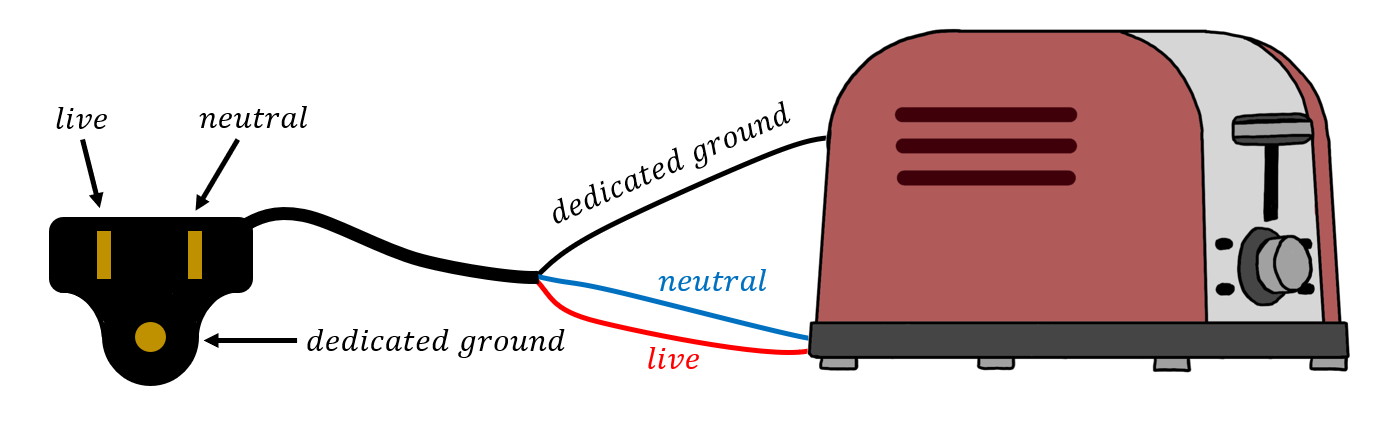
\includegraphics[width=1\linewidth]{files/toaster-1f623c53aaf6f4b9b0a91566c6ecca0d.png}
\caption[]{When an appliance has three prongs on its electrical cable, the middle prong grounds the case to the dedicated ground as a safety measure. Note that the live wire is not necessarily the right-hand side socket on an outlet!}
\label{fig:current:toaster}
\end{figure}

\subsubsection{Summary}

Electric current, $I$, is defined as the rate at which charges cross some plane (for example a plane perpendicular to a wire) per unit time. That is, if an amount of charge, $\Delta Q$, enters a wire during an amount of time, $\Delta t$, the current, $I$, in that wire is defined to be:
\begin{equation}
I=\frac{\Delta Q}{\Delta t}=\frac{dQ}{dt}
\end{equation}
where a derivative is taken if the rate at which charges are moving is not constant with time.

Electric current is a macroscopic quantity that can be measured. Conventional current is defined to be positive in the direction in which positive charges flow. In most situations, it is electrons that move inside a conductor, so the current is defined to be positive in the \textit{opposite direction} of the actual motion of the (negative) electrons.

The current density, $\vec j$, is defined to be the current per unit area at some point in a conductor, and is a vector in the direction of the electric field, $\hat E$, at that point:
\begin{equation}
\vec j = \frac{I}{A}\hat E
\end{equation}
The current density can be related to the microscopic motion of charges within the conductor. If the current density, $\vec j$, is known, the corresponding current, $I$, that crosses a surface with area, $A$, and normal vector, $\hat n$, is given by:
\begin{equation}
I=A \vec j\cdot \hat n=\int \vec j \cdot d\vec A
\end{equation}
where the integral must be taken if the current density is not constant over the surface.

A conducting material through which current is flowing is called a resistor. When a potential difference is applied across a resistor, the resulting electric field will drive the flow of electrons through the resistor. The electrons will flow with an average ``drift velocity'', $\vec v_d$, which is much lower than the actual (Fermi) speed of the electrons in the material. Inside the resistor, electrons are constantly accelerated before they collide with atoms in the material losing their kinetic energy, and then accelerating again. Thus, the potential energy that is available to the electrons is ``used'' to heat the resistor, and the electrons, on average, drift quite slowly through the resistor.

The current density in a resistor can be related to the drift velocity of the electrons and the ``density of free electrons'' in the material, $n$:
\begin{equation}
\vec j = -en\vec v_d
\end{equation}
where, $e$,  is the magnitude of the charge of the electrons and the minus sign indicates that the current density is in the opposite direction of the velocity of the (negative) electrons.

Ohm's Law states that the current density, $\vec j$, at some point in the conductor is proportional to the electric field, $\vec E$, at that point:
\begin{equation}
\vec j=\sigma \vec E=\frac{1}{\rho}\vec E
\end{equation}
where the constant of proportionality, $\sigma$, is called the ``conductivity'' of the material (and is a property of the material through which current is flowing). The resistivity, $\rho$, is a material property that is simply the inverse of the conductivity. Both of these properties are a measure of how large a current (or current density) will exist in a material given a certain electric field. For example, the conductivity of an insulating material is close to zero (and its resistivity close to infinity).

For most materials, resistivity usually increases linearly with temperature:
\begin{equation}
\rho(T)=\rho_0[1+\alpha(T-T_0)]
\end{equation}
where $\rho_0$ is the resistivity as measured at some reference temperature, $T_0$ (usually $20 {\rm \degree C}$), and $\alpha$, is the ``temperature coefficient'' for that material. Note that this model of resistivity does not hold for extreme temperatures (very cold or very hot), and for some materials, resistivity decreases with temperature ($\alpha$ is negative).

If we apply Ohm's Law to a resistor of length, $L$, cross-sectional area, $A$, made of a material with resistivity, $\rho$, we find that the potential difference applied across the resistor, $\Delta V$, is proportional to the current flowing through the resistor:
\begin{equation}
\Delta V =\rho \frac{L}{A} I
\end{equation}
The constant of proportionality depends on the material with which the resistor is made (through the resistivity) and on the dimensions of the resistor (through the length and cross-sectional area). The constant of proportionality is called the ``resistance'' of the resistor, $R$:
\begin{equation}
R=\rho \frac{L}{A}
\end{equation}
Ohm's Law is often written for a resistor as the relationship between the current through the resistor, $I$, and the potential difference across the resistor, $\Delta V$:
\begin{equation}
\Delta V = RI
\end{equation}
although, technically, Ohm's Law is the relation between current density and electric field.

Resistors can be combined in series, in which case, the effective resistance of the combination is found by adding the resistances of the individual resistors:
\begin{equation}
R_{eff}=R_1+R_2+R_2+\dots\quad\text{(Series resistors)}
\end{equation}
When combined in parallel, the inverse of the effective resistance is given by the inverse of the sum of the inverse of the resistances of the individual resistors:
\begin{equation}
R_{eff}=\frac{1}{\frac{1}{R_1}+\frac{1}{R_2}+\frac{1}{R_3}+\dots}\quad\text{(Parallel resistors)}
\end{equation}

As charges move through a resistor of resistance, $R$, under a potential difference, $\Delta V$, and current, $I$, they transfer their kinetic energy into heating up the resistor. The rate at which they transfer the energy, also called the ``power dissipated in the resistor'', is given by:
\begin{equation}
P=I \Delta V=\frac{(\Delta V)^2}{R}=I^2R
\end{equation}
where the various combinations can be obtained by applying the macroscopic version of Ohm's Law.

The electrical outlets in our daily lives provide an ``alternating'' voltage, $\Delta V(t)$, which oscillates sinusoidally:
\begin{equation}
\Delta V(t)=\Delta V_0\sin(\omega t)
\end{equation}
with a maximum amplitude, $\Delta V_0$, and an angular frequency, $\omega = 2\pi f$. When this potential difference is applied across a resistor, an alternating current is formed, in which the electrons move back and forth, with no net displacement:
\begin{equation}
I(t)=\frac{\Delta V_0}{R}=I_0\sin(\omega t)
\end{equation}
Even though there is not net displacement, the electrons will still transfer energy into the resistor in the form of heat. The average rate at which power is dissipated in the resistor is given by:
\begin{equation}
\bar P=\frac{1}{2}RI_0^2
\end{equation}
We introduce the ``root mean square'' current (voltage), $I_{rms}$ ($\Delta V_{rms}$), as an average effective current (voltage):
\begin{equation}
I_{rms}&=\frac{1}{\sqrt 2}I_0\\
\Delta V_{rms}&=\frac{1}{\sqrt 2}\Delta V_0
\end{equation}
such that the power can be expressed using a similar formula as in the direct current case, using the root mean square values:
\begin{equation}
\bar P = I_{rms}^2R = I_{rms}\Delta V_{rms}=\frac{(\Delta V_{Rms})^2}{R}
\end{equation}
There are two main types of hazards associated with the use of electricity: fire and electrocution. Electrical fires can arise when a large current goes through a wire, since this will dissipate a large amount of heat into the wire (which could set fire to its insulation or other nearby flammable items). Electrocution occurs when a current traverses the human body. If a current above $\sim80 {\rm mA}$ crosses the upper body, this can result in ventricular fibrillation, whereby the heart beats very irregularly. Of course, one can also be burned by a large current. The amount of current through the body is what will ultimately determine the severity of injuries, and is why one often hears that ``it's current that kills''. A large voltage may not lead to a large current if the resistance of the person is large or if the power supply cannot provide a large current at that large voltage.

\begin{framed}
\textbf{Important Equations}\\
\textbf{Current:}
\begin{equation}
I = \frac{\Delta Q}{\Delta t}=\frac{dQ}{dt}
\end{equation}

\textbf{Current density:}
\begin{equation}
\vec j = \frac{I}{a}\hat E \\
I = \int \vec j \cdot d \vec A
\end{equation}

\textbf{Microscopic model of current:}
\begin{equation}
\vec j = -en \vec v_d
\end{equation}

\textbf{Ohm's Law:}
\begin{equation}
\vec j = \sigma \vec E
\end{equation}

\textbf{Resistivity:}
\begin{equation}
\rho = \frac{1}{\sigma}\\
\rho(T)=\rho_0[1+\alpha(T-T_0)]
\end{equation}

\textbf{Resistance:}
\begin{equation}
R = \rho \frac{L}{A}
\end{equation}

\textbf{Ohm's Law (macroscopic):}
\begin{equation}
\Delta V = R I
\end{equation}

\textbf{Combining resistors:}
\begin{equation}
R_{eff}&=R_1+R_2+R_2+\dots\quad\text{(Series)}\\
R_{eff}&=\frac{1}{\frac{1}{R_1}+\frac{1}{R_2}+\frac{1}{R_3}+\dots}\quad\text{(Parallel)}
\end{equation}
\textbf{Power dissipated in a resistor:}
\begin{equation}
P=I \Delta V=\frac{(\Delta V)^2}{R}=I^2R
\end{equation}

\textbf{RMS voltage and current:}
\begin{equation}
I_{rms}&=\frac{1}{\sqrt 2}I_0\\
\Delta V_{rms}&=\frac{1}{\sqrt 2}\Delta V_0
\end{equation}
\end{framed}

\begin{framed}
\textbf{Important Definitions}\\
\begin{itemize}
\item \textbf{Current:} The rate at which charges flow across a given surface. SI units: ${\rm \left[{A}\right]}$. Common variable(s): $I$.
\item \textbf{Current density:} A measure of current per unit area, in the direction of the local electric field. SI units: ${\rm \left[{Am^{ -1}}\right]}$. Common variable(s): $\vec j$.
\item \textbf{Resistance:} A measure of a specific object's opposition to the flow of charge. SI units: ${\rm \left[{\Omega}\right]}$. Common variable(s): $R$.
\item \textbf{Resistivity:} A measure of a material's opposition to the flow of charge. SI units: ${\rm \left[{\Omega m}\right]}$. Common variable(s): $\rho$.
\item \textbf{Conductivity:} The inverse of resistivity. SI units: ${\rm \left[{\Omega^{ -1} m^{ -1}}\right]}$. Common variable(s): $\sigma$.
\item \textbf{Drift velocity:} The average velocity of an electron drifting in a conductor under the influence of an electric field. SI units: ${\rm \left[{ms^{ -1}}\right]}$. Common variable(s): $\vec v_{d}$.
\end{itemize}
\end{framed}

\subsubsection{Thinking about the material}

\begin{framed}
\textbf{Reflect and research}\\
\begin{itemize}
\item Describe how superconductivity arises in certain materials (hint: research ``Cooper pairs'').
\item What are some example of superconducting materials, and at what temperature do they become superconducting?
\item Is there a limit to how much current a conductor can carry?
\item Does an AC current have a drift velocity? Why or why not?
\end{itemize}
\end{framed}

\begin{framed}
\textbf{To try at home}\\
\begin{itemize}
\item Use Ohm's law and the electrical information on an appliance to determine the current produced drawn by your appliance (e.g. a hair dryer).
\item What is the current produced by your phone's battery? What is the total power stored in your phone's battery? Check the technical information of your phone.
\end{itemize}
\end{framed}

\begin{framed}
\textbf{To try in the lab}\\
\begin{itemize}
\item Propose an experiment to create an AC circuit and measure its current.
\item Propose an experiment to measure the temperature coefficient ($\alpha$) and resistivity of a wire.
\end{itemize}
\end{framed}

\subsubsection{Sample problems and solutions}

\paragraph{Problems}

\begin{framed}
\textbf{Problem 18.1}\\
A cylindrical wire of radius $R$ has a current density that increases with radius as $\vec j(r) = ar \vec z$, where $r$ is the radial distance from the centre of the wire, $a$ is a constant, and $\vec z$ is normal to the face of the cylinder. What is the total current in the wire?
\end{framed}

\begin{framed}
\textbf{Problem 18.2}\\
A resistor is measured to have a resistance of $R_1=103.4 {\rm \Omega}$ at a temperature of $T_1=30 {\rm \degree C}$, and a resistance of $R_2=106.8 {\rm \Omega}$ at a temperature of $T_2=40 {\rm \degree C}$. Using the values in Table~\ref{tab:current:materials}, determine the material from which the resistor is made.
\end{framed}

\paragraph{Solutions}

\begin{framed}
\textbf{Solution 18.1}\\
To determine the current through the entire cross section of the wire, we first divide the cross-section of the wire into infinitesimally small concentric rings of radius, $r$, and width, $dr$. The cross-sectional area of one ring is given by:
\begin{equation}
d\vec A = 2\pi r dr \vec z
\end{equation}
so that the current through one ring is given by:
\begin{equation}
dI = j(r) dA = 2\pi a r^2 dr
\end{equation}
The current through the whole wire is then found by summing the currents through each ring:
\begin{equation}
I=\int dI = \int_0^R 2\pi a r^2 dr=\frac{2}{3}\pi aR^3
\end{equation}
\end{framed}

\begin{framed}
\textbf{Solution 18.2}\\
To determine the material of the resistor, we can find the temperature coefficient, $\alpha$, since we are given measurements of resistance, $R_1$ and $R_2$, at two different temperatures, $T_1$, and $T_2$, respectively. The reference temperature is set to be $T_0=20 {\rm \degree C}$, so that we can compare with Table~\ref{tab:current:materials}.

We know that the resistance will vary with temperature, since the resistivity is temperature-dependent. The temperature dependence of resistivity is given by:
\begin{equation}
\rho(T)=\rho_0[1+\alpha(T-T_0)]
\end{equation}
If the resistor has length, $L$, and cross-sectional area, $A$, it will have resistance, $R$, given by:
\begin{equation}
R(T)=\rho(T) \frac{L}{A}=\frac{\rho_0 L}{A}[1+\alpha(T-T_0)]=R_0[1+\alpha(T-T_0)]
\end{equation}
where $R_0$ is the resistance at the reference temperature, $T_0$. Since we are given the resistance at two different temperatures, we can determine both $\alpha$ and $R_0$, for a choice of $T_0=20 {\rm \degree C}$:
\begin{equation}
R_1&=R_0[1+\alpha(T_1-T_0)]\\
R_2&=R_0[1+\alpha(T_2-T_0)]\\
\therefore\frac{R_1}{R_2}&=\frac{1+\alpha(T_1-T_0)}{1+\alpha(T_2-T_0)}\\
R_1 [1+\alpha(T_2-T_0)]&=R_2 [1+\alpha(T_1-T_0)]\\
\alpha \left( R_1(T_2-T_0) - R_2(T_2-T_0) \right)&=R_2-R_1\\
\therefore \alpha &= \frac{R_2-R_1}{R_1(T_2-T_0) - R_2(T_1-T_0) }\\
&=\frac{(106.8 {\rm \Omega}) - (103.4 {\rm \Omega})}{(103.4 {\rm \Omega})((40 {\rm \degree C})-(20 {\rm \degree C})) - (106.8 {\rm \Omega})((30 {\rm \degree C})-(20 {\rm \degree C})) }\\
&=0.0034
\end{equation}
Referring to Table~\ref{tab:current:materials}, the material could likely be gold.
\end{framed}

% %%You have your washing machine, television, and dish washer connected to the same circuit. You would like to use the vacuum, but aren't sure if it will draw too much power... (rest of power dissipation question...) %could be a QL question?
% %%